\title{Internship defense}
\subtitle{Fullstack developer at Doctolib}
\author{Victor Schubert}
\date{2018--11--16}

\frame{\titlepage}

\begin{frame}
	\frametitle{What is Doctolib?}
	Created by Stan Niox-Ch\^ateau, Ivan Schneider and Jessy Bernal in 2013
	\begin{itemize}[<+->]
		\item 650 collaborators in France and Germany
		\item 65,000 practitioners paying 109\euro/month each
		\item 25,000,000 visits each month
		\item 3000 requests each seconds \only<6->{on monday mornings}
	\end{itemize}
\end{frame}

\begin{frame}
	\frametitle{But\dots What {\em is} Doctolib?}
	\begin{itemize}[<+->]
		\item 120,000 lines of code
		\item 60,000 lines of test
		\item 8,500 tests
		\item 30 developers \only<5->{and growing}
		\item<6-> no downtime in the last three months
		\item<7-> {\em one} monolith
		\item<8-> no nonsense
	\end{itemize}
\end{frame}

\begin{frame}
	\frametitle{But\dots What {\em is} Doctolib?}
	\centering
	\begin{tikzpicture}[node distance=0.6,text height=.90em,text depth=.30em]
		\node (inet) [rectangle]                 {Internet};
		\node (flar) [minimum width=11em,draw,rectangle,below=of inet] {Cloudflare};
		\node (rora) [minimum width=11em,draw,rectangle,below=of flar] {Ruby on Rails};
		\node (psql) [minimum width=11em,draw,rectangle,below=of rora] {PostgreSQL};
		\node (srvr) [minimum width=11em,draw,rectangle,below=of psql] {Dedicated servers};
		\node [rectangle,below=of srvr] {\small no nonsense};
		\draw (inet) edge (flar);
		\draw (flar) edge (rora);
		\draw (rora) edge (psql);
		\draw (psql) edge (srvr);
	\end{tikzpicture}
\end{frame}

\begin{frame}
	\frametitle{Who do I work with?}
	\centering
	\begin{tabular}{>{\bfseries}ll}
		\multicolumn{2}{l}{\bfseries The Patient feature team} \\
		\hline
		Micka\"el Morier & Developer \\
		M\'elanie Godard & Developer \\
		M\'elanie B\'erard & Developer \\
		Victor Schubert & Developer \\
		Paul Doidge & Engineering manager \\
		Renan Le Gall & Product owner \\
		Jean-Baptiste Cazaux & Developer \\
		Timoth\'ee Le Borgne & Product owner \\
		Aur\'elien Pieropan & Developer \\
	\end{tabular}
\end{frame}

\begin{frame}
	\frametitle{What is the Tech Holder?}
	\centering
	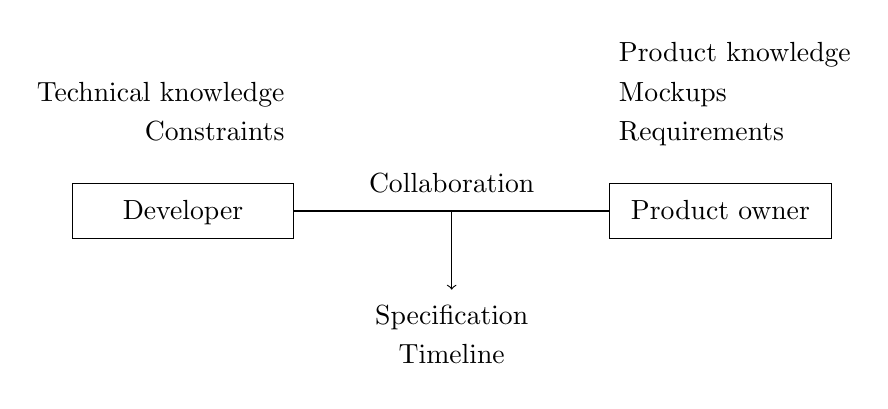
\begin{tikzpicture}[node distance=0.6,text height=.90em,text depth=.30em]
		\node (th) at (-2, 0) [draw,rectangle,anchor=east,minimum height=2em,minimum width=8em] {Developer};
		\node (po) at (2, 0) [draw,rectangle,anchor=west,minimum height=2em,minimum width=8em] {Product owner};
		\node at (0, 0) [anchor=south] {Collaboration};
		\draw (th)--(po);
		\draw (0, 0)[->]--(0, -1);
		\node at (0, -1) [anchor=north] {Specification};
		\node at (0, -1.5) [anchor=north] {Timeline};
		\node at (-2, 1) [anchor=east] {Constraints};
		\node at (-2, 1.5) [anchor=east] {Technical knowledge};
		\node at (2, 1) [anchor=west] {Requirements};
		\node at (2, 1.5) [anchor=west] {Mockups};
		\node at (2, 2) [anchor=west] {Product knowledge};
	\end{tikzpicture}
\end{frame}

\begin{frame}
	\frametitle{What is the Tech Holder?}
	Before the sprint starts:
	\begin{enumerate}[<+->]
		\item Understand the project
		\item Define Key Performance Indicators
		\item Identify technical risks
		\item Identify organizational risks
		\item Check-in with the legal team
		\item Check-in with the infosec team
		\item Roughly size the project
		\item Split it if necessary
		\item Draft a specification for the implementation
	\end{enumerate}
\end{frame}

\begin{frame}
	\frametitle{What is the Tech Holder?}
	During the sprint:
	\begin{itemize}[<+->]
		\item Coordinate the development team
		\item Know the big picture
		\item Update the timeline
		\item Communicate on these updates!
	\end{itemize}
\end{frame}

\begin{frame}
	\frametitle{What is the Tech Holder?}
	After the rollout:
	\begin{itemize}[<+->]
		\item Own the codebase for the project
		\item Measure the project's impact
		\item Be a reference for this project
	\end{itemize}
\end{frame}

\begin{frame}
	\vfill
	\centering
	\includegraphics[width=0.5\textwidth]{\doctolibLogo}
	\vfill
\end{frame}
% vim: set ts=3 sts=3 sw=3 noet syntax=tex:
